\documentclass[11pt, a4paper]{article}
\font\myfont=cmr12 at 41pt
\title{{\myfont Combinatorial Proof}}
\date{13-08-2019}
\author{Claudiu Rediu}
\usepackage[margin=1.5in]{geometry}
\usepackage{hyperref}
\usepackage[utf8]{inputenc}
\usepackage[english]{babel}
\usepackage{amsthm}
\usepackage{amssymb}
\usepackage{amsmath}
\usepackage{graphicx}
\renewcommand\qedsymbol{$\blacksquare$}
\usepackage{float}
\theoremstyle{definition}
\newtheorem*{definition}{Definition} %the * is such that the definition are not numbered
\theoremstyle{theorem}
\newtheorem*{theorem}{Theorem}

\begin{document}
	\pagenumbering{gobble}
	\maketitle
	\newpage
	\pagenumbering{arabic}
	\newpage
	\begin{theorem}
		For m,n,k non-negative integers $\sum_{k=0}^{n}\binom{n}{k}\binom{k}{m} = \binom{n}{m}2^{n-m}$
	\end{theorem}

	\begin{proof}
	In terms of combinations, $\sum_{k=0}^{n}\binom{n}{k} = 2^n$ is the sum of the nth row (counting from 0) of the binomial coefficients in the Pascal's triangle (Figure \ref{fig:pascals}). 
	
	Let's take first $ m = 1 $ for which $\sum_{k=1}^{n}k\binom{n}{k} = n2^{n-1}$ is a more simple case. What does this mean?
	
	On the left-hand side, it is similar to the triangle being $n-1$ in size. This results in $2^{n-1}$ combinations. Multiplying this by $k$ gives $$\sum_{k=1}^{n}k\binom{n}{k} = n2^{n-1}$$ Increasing the number of rows omitted to $m \le n$ would result in $\binom{n}{m}$ binomial coefficients in the Pascal triangle of size $n-m$. 
	This is equal to the right-hand side of the equations. This means that the equation is valid and
	$$\sum_{k=0}^{n}\binom{n}{k}\binom{k}{m} = \binom{n}{m}2^{n-m}$$
	\end{proof}
	\begin{figure}[h]
		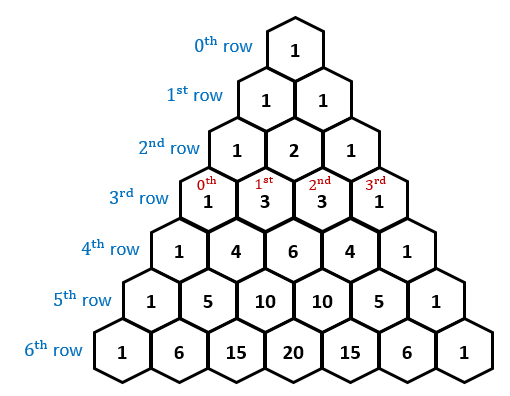
\includegraphics[width = \linewidth, height = 250px]{pascals.png}
		\caption{Representation of Pascal's triangle}
		\label{fig:pascals}
	\end{figure}
	
\end{document}